\section{多重校验纠错}
\label{chap:hash:robustness}

本节对该方法中的多重校验纠错展开介绍,分别为基于HASH的码字间校验方法、基于CRC的码字自校验方法,以及基于异或校验的映射矩阵校验方法。各方法的展开介绍,包括调制阶段及解调阶段两个方面。

\subsection{基于HASH的码字间校验方法}
\label{chap:hash:robustness:hash}

基于HASH的码字间校验方法,涉及到的参数为$L_{HASH}$及$R$、用户共享的$Salt$及RTP中导出的随机$Seed$。通过建立多组码字之间的校验关系,建立码字间的级联校验。

\subsubsection{调制阶段}
\label{chap:hash:robustness:hash:modulation}

\insertFigure{
	\begin{figure}[htbp]
		\centering
        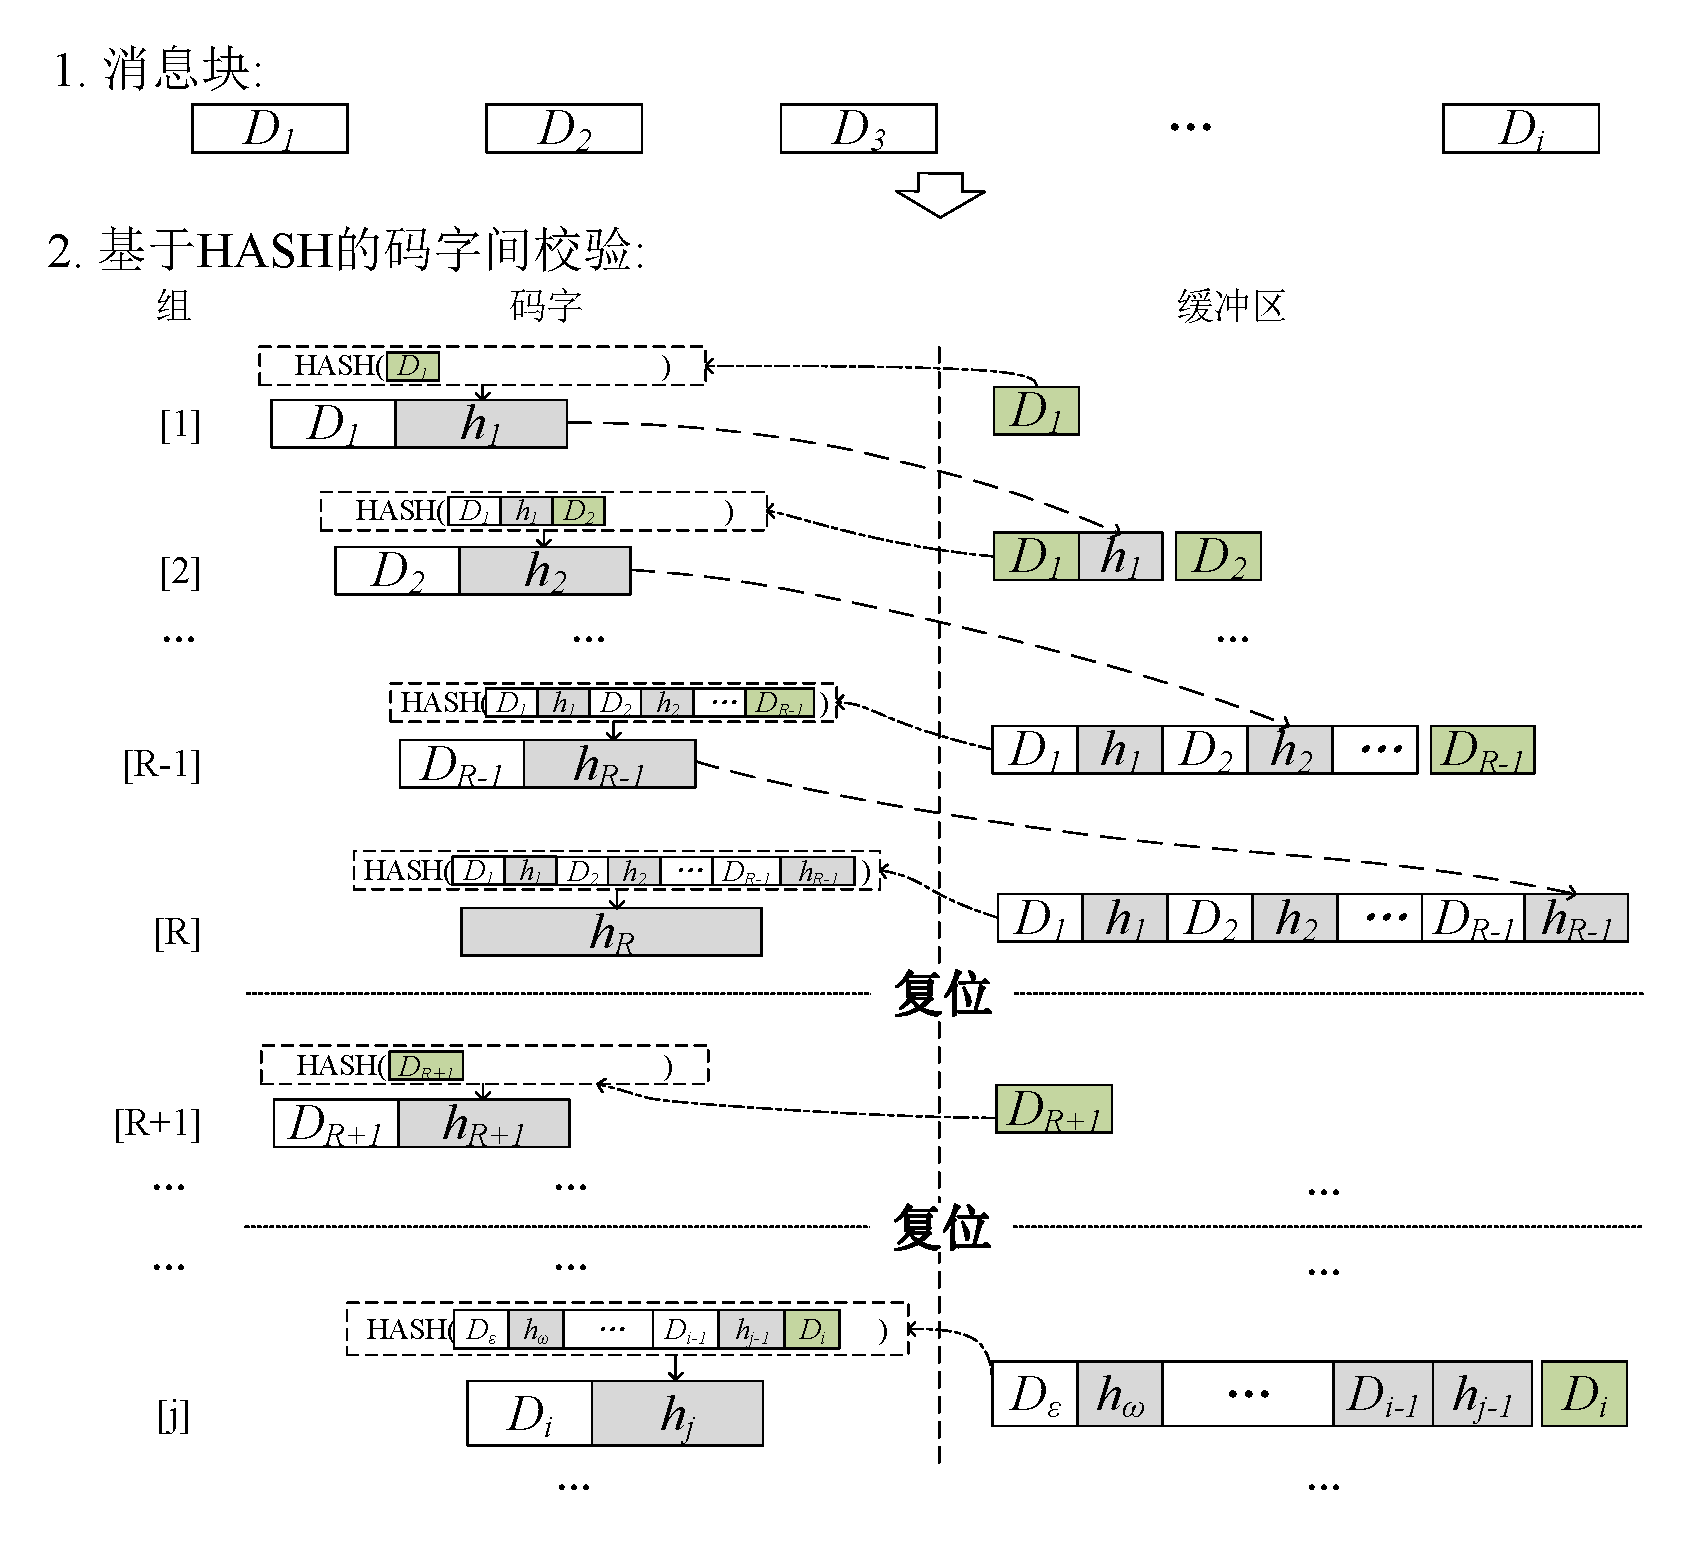
\includegraphics[width=0.9\textwidth]{chapters/chapter5/figures/hash-chain.pdf}
        \caption{基于HASH的码字间校验调制阶段示意图}
        \label{fig:5:hash-chain}
    \end{figure}
}
\insertEquation{
    \begin{equation}
        \label{equ:5:omega-j}
        \omega\ =\ {\left \lfloor{\frac{j\ -\ 1}{R}}\right \rfloor}\ \times\ {R\ +\ 1}
    \end{equation}
    \begin{equation}
        \label{euq:5:varepsilon-omega}
        \varepsilon\ =\ \omega\ -\ {\left \lfloor{\frac{\omega}{R}}\right \rfloor}
    \end{equation}
    \begin{equation}
        \label{euq:5:i-j}
        i\ =\ j\ -\ {\left \lfloor{\frac{j}{R}}\right \rfloor}
    \end{equation}
    \begin{equation}
        \label{euq:5:j-i}
        j\ =\ \left \lfloor{\frac{i}{R\ -\ 1}} \right \rfloor\ \times\ R\ +\ (i\ -\ 1)\ \%\ R\ +\ 1
    \end{equation}
}

调制阶段,基于HASH的码字间校验如图\ \nref{fig:5:hash-chain}。建立码字间的级联校验,需要维持发送缓冲区,用于记录当前待校验的内容。起始阶段缓冲区为空,将第一组的数据块$D_{1}$添加到缓冲区中,并计算HASH$(D_{1})$作为$h_{1}$拼接到$D_{1}$末尾,同时将$h_{1}$添加到缓冲区。按照组号顺序,依次迭代校验过程。当组号为$R$时,缓冲区中数据已经累计得足够长,执行复位操作。复位阶段,生成特殊的校验块$h_{R}$,其长度为$BL\ +\ L_{HASH}$,并将缓冲区清空。

按照复位周期$R$,依次计算所有的码字间校验块$h_{j}$,直至到达末尾。由于复位阶段添加了额外的校验码字,$D_{i}$与$h_{j}$中$i$与$j$的对应关系如公式(\nref{euq:5:j-i})及公式(\nref{euq:5:i-j})。图\ \nref{fig:5:hash-chain}中,复位后的起始消息块$D_{\varepsilon}$与组号$j$的关系,如公式(\nref{euq:5:varepsilon-omega})及公式(\nref{equ:5:omega-j})。

\subsubsection{解调阶段}
\label{chap:hash:robustness:hash:demodulation}

\insertFigure{
    \begin{figure}[htbp]
        \centering
        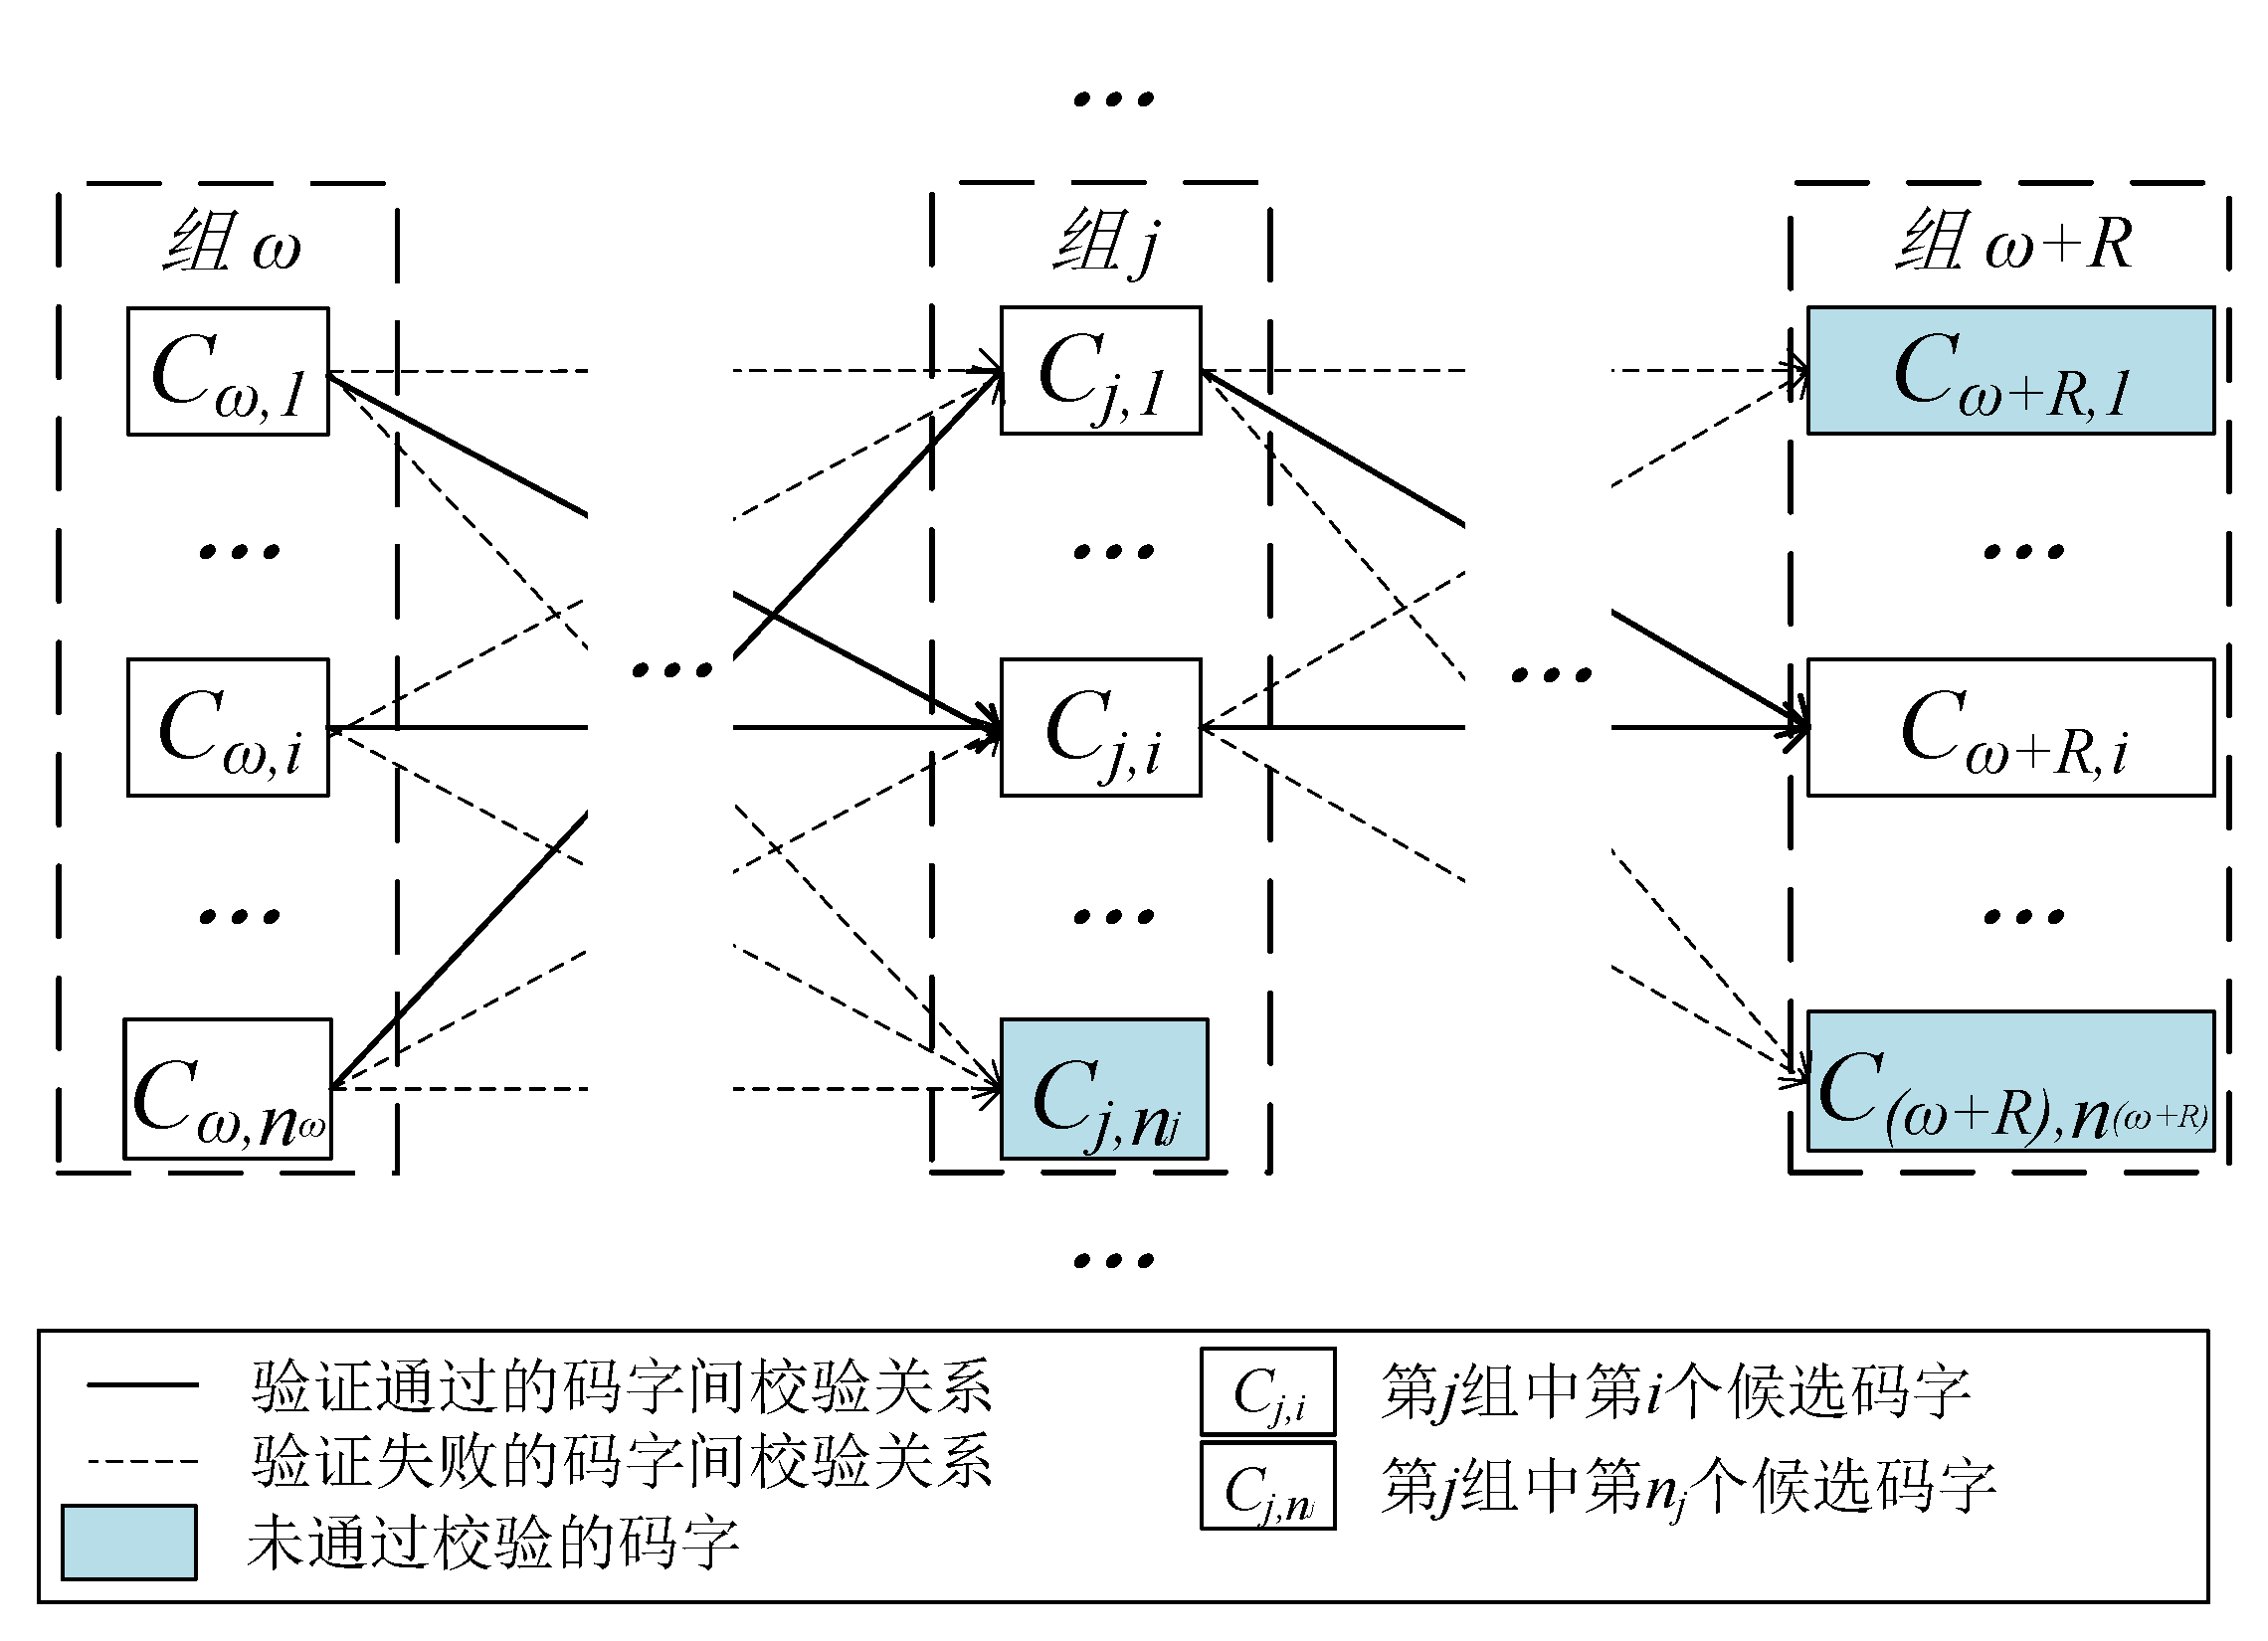
\includegraphics[width=0.8\textwidth]{chapters/chapter5/figures/hash-verification.pdf}
        \caption{基于HASH的码字间校验解调阶段示意图}
        \label{fig:5:hash-verification}
    \end{figure}
}

解调阶段,基于HASH的码字间校验如图\ \nref{fig:5:hash-verification},按照复位周期$R$进行切分,每个周期内的验证过程单独进行,在减小计算规模的同时防止噪声传播。对于每个周期内的候选码字集合$\{\{C_{1}',\ \cdots\},\ \{C_{2}',\ \cdots \},\ \cdots ,\ \{C_{R}',\ \cdots\}\}$,所有的可行解构成了一个有向无环图,图的起点为$\{C_{1}',\ \cdots \}$,图中的每条边对应了一种码字间关联关系。

解调过程与图遍历过程类似,由起点开始,对所有的边进行验证。只有符合校验规则时,才保留,否则将边由图中删除。对于非$\omega\ +\ R$组的节点,当节点出度为0时,意味着没有满足要求的后继节点,判断该节点为网络噪声并移除。最终,当存在一条由起点出发的路径达到第$\omega\ +\ R$组的节点,即为一种可能的码字组合。在网络噪声干扰下,候选组合不唯一,选择所有路径中节点入度之和最大的一条路径,作为最终结果。

\subsection{基于CRC的码字自校验方法}
\label{chap:hash:robustness:crc}

\insertContents{
    \begin{algorithm}[htbp]
        \renewcommand{\algorithmcfname}{算法}
        \caption{码字生成}
        \label{alg:5:codeword-generation}
        \LinesNumbered
        \KwIn{$message$,\ $BL$,\ $L_{HASH}$,\ $L_{CRC}$,\ $R$,\ $Salt$,\ $Seed$}
        \KwOut{$C\ \leftarrow\ \{\}$}
        $D\ \leftarrow$\ group into blocks$(message,\ BL)$ \\
        $modulated\_sections\ \leftarrow\ NULL$ \\
        $salt\ \leftarrow\ Salt\ \oplus\ Seed$ \\
        \For {$D_i$\ in\ $D$} {
            $j\ \leftarrow\ \left \lfloor{\frac{i}{R\ -\ 1}} \right \rfloor\ \times\ R\ +\ (i\ -\ 1)\ \%\ R\ +\ 1$ \\
            append\ $D_i$\ to\ $modulated\_sections$ \\
            $h_j\ \leftarrow\ L_{HASH}$\ bits\ of\ HASH\ ($salt\ //\ modulated\_sections\ //\ salt$) \\
            $C_j\ \leftarrow$\ append\ $h_j$\ to\ $D_i$ \\
            append\ $h_j$\ to\ $modulated\_sections$ \\
            append\ $C_j$\ to\ $C$ \\
            \If {$i$\ mod\ $R$\ ==\ 0} {
                $C_{j+1}\leftarrow (L_{Codeword} - L_{CRC})$\ bits of HASH($salt//modulated\_sections//salt$) \\
                append\ $C_{j\ +\ 1}$\ to\ $C$ \\
                $modulated\_sections\ \leftarrow\ NULL$ \\
            }
        }
        \For {$C_j$ in $C$} {
            $C_j\ \leftarrow$\ append\ $L_{CRC}$\ bits of CRC32\ ($salt\ //\ C_j\ //\ salt$)\ to\ $C_j$
        }
        \Return $C$
    \end{algorithm}
}


基于CRC的码字自校验方法,通过在码字$C_{j}$中设置CRC校验块$v_{j}$,验证$D_{i}\ //\ h_{j}$部分的正确性。该校验方法基于单个码字,不存在码字间的依赖关系,因此调制及解调过程效率较高。

\subsubsection{调制阶段}
\label{chap:hash:robustness:crc:modulation}

\insertFigure{
	\begin{figure}[htbp]
		\centering
        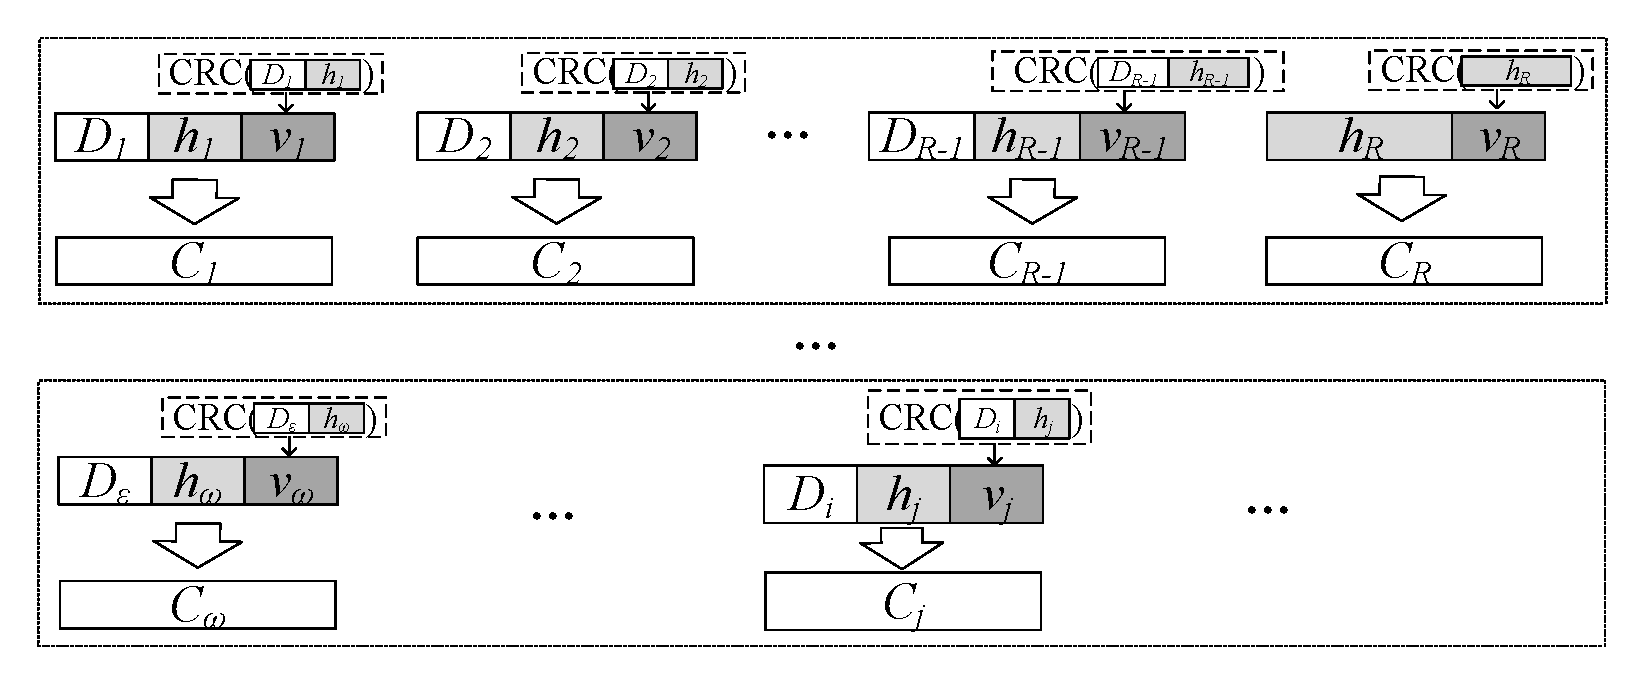
\includegraphics[width=0.8\textwidth]{chapters/chapter5/figures/crc-generation.pdf}
        \caption{基于CRC的码字自校验调制阶段示意图}
        \label{fig:5:crc-generation}
    \end{figure}
}

调制阶段,基于CRC的码字间自校验过程如图\ \nref{fig:5:crc-generation}。码字由$D_{i}$、$h_{j}$及$v_{j}$三部分组成,基于CRC的码字校验块即$v_{j}$,$v_{j}$为CRC散列结果中的{$L_{CRC}$\ bits}。

基于CRC的码字自校验计算完毕后,码字的各组成部分均完备,组合即可得到码字$C_{j}$。算法\ \nref{alg:5:codeword-generation}描述了由隐蔽消息到码字的处理过程,包含消息分组及码字生成两个部分。计算HASH摘要及CRC散列值过程中,均进行了加盐操作,保证校验信息的随机性。

\subsubsection{解调阶段}
\label{chap:hash:robustness:crc:demodulation}

\insertContents{
    \begin{algorithm}[htb]
        \renewcommand{\algorithmcfname}{算法}
        \caption{有效码字鉴别}
        \label{alg:5:codeword-identification}
        \LinesNumbered
        \KwIn{$S'$,\ $L_{CRC}$,\ $Salt$,\ $Seed$}
        \KwOut{$C'\ \leftarrow\ \{\}$}
        $salt\ \leftarrow\ Salt\ \oplus\ Seed$ \\
        \For {\{${S_j'}$\}\ in\ $S'$} {
            $\{C_j'\}\ \leftarrow\ \{\}$ \\
            \For {$S_j'$\ in\ \{$S_j'$\}} {
                $v_j',\ h_j',\ D_j'\ \leftarrow$\ extracted from $S_j'$ \\
                $crc32\_result\ \leftarrow\ L_{CRC}$ bits of CRC32\ ($salt\ //\ D_j'\ //\ h_j'\ //\ salt$) \\
                \If {$v_j'$ == $crc32\_result$} {
                    append\ $S_j'$\ to\ \{$C_j'$\}
                }
            }
            append\ \{$C_j'$\}\ to\ $C'$
        }
        \Return $C'$
    \end{algorithm}
}

基于CRC的码字自校验解调阶段的描述如算法\ \nref{alg:5:codeword-identification},对于候选符号,只有符合校验规则才导出为候选码字。解调过程重新计算CRC校验值,判断与码字的$v_{j}'$部分是否一致,不一致则直接丢弃。解调过程中,采取的加盐方式及取值与调制过程保持一致。

\subsection{基于异或的映射矩阵校验方法}
\label{chap:hash:robustness:xor}

映射矩阵实现了码字到数据包序号的转换,并在矩阵内部实现了基于异或校验的符号校验,同时矩阵的列数为可调整的参数,有利于降低连续丢包噪声的干扰。

\subsubsection{调制阶段}
\label{chap:hash:robustness:xor:modulation}

\insertFigure{
	\begin{figure}[htb]
		\centering
        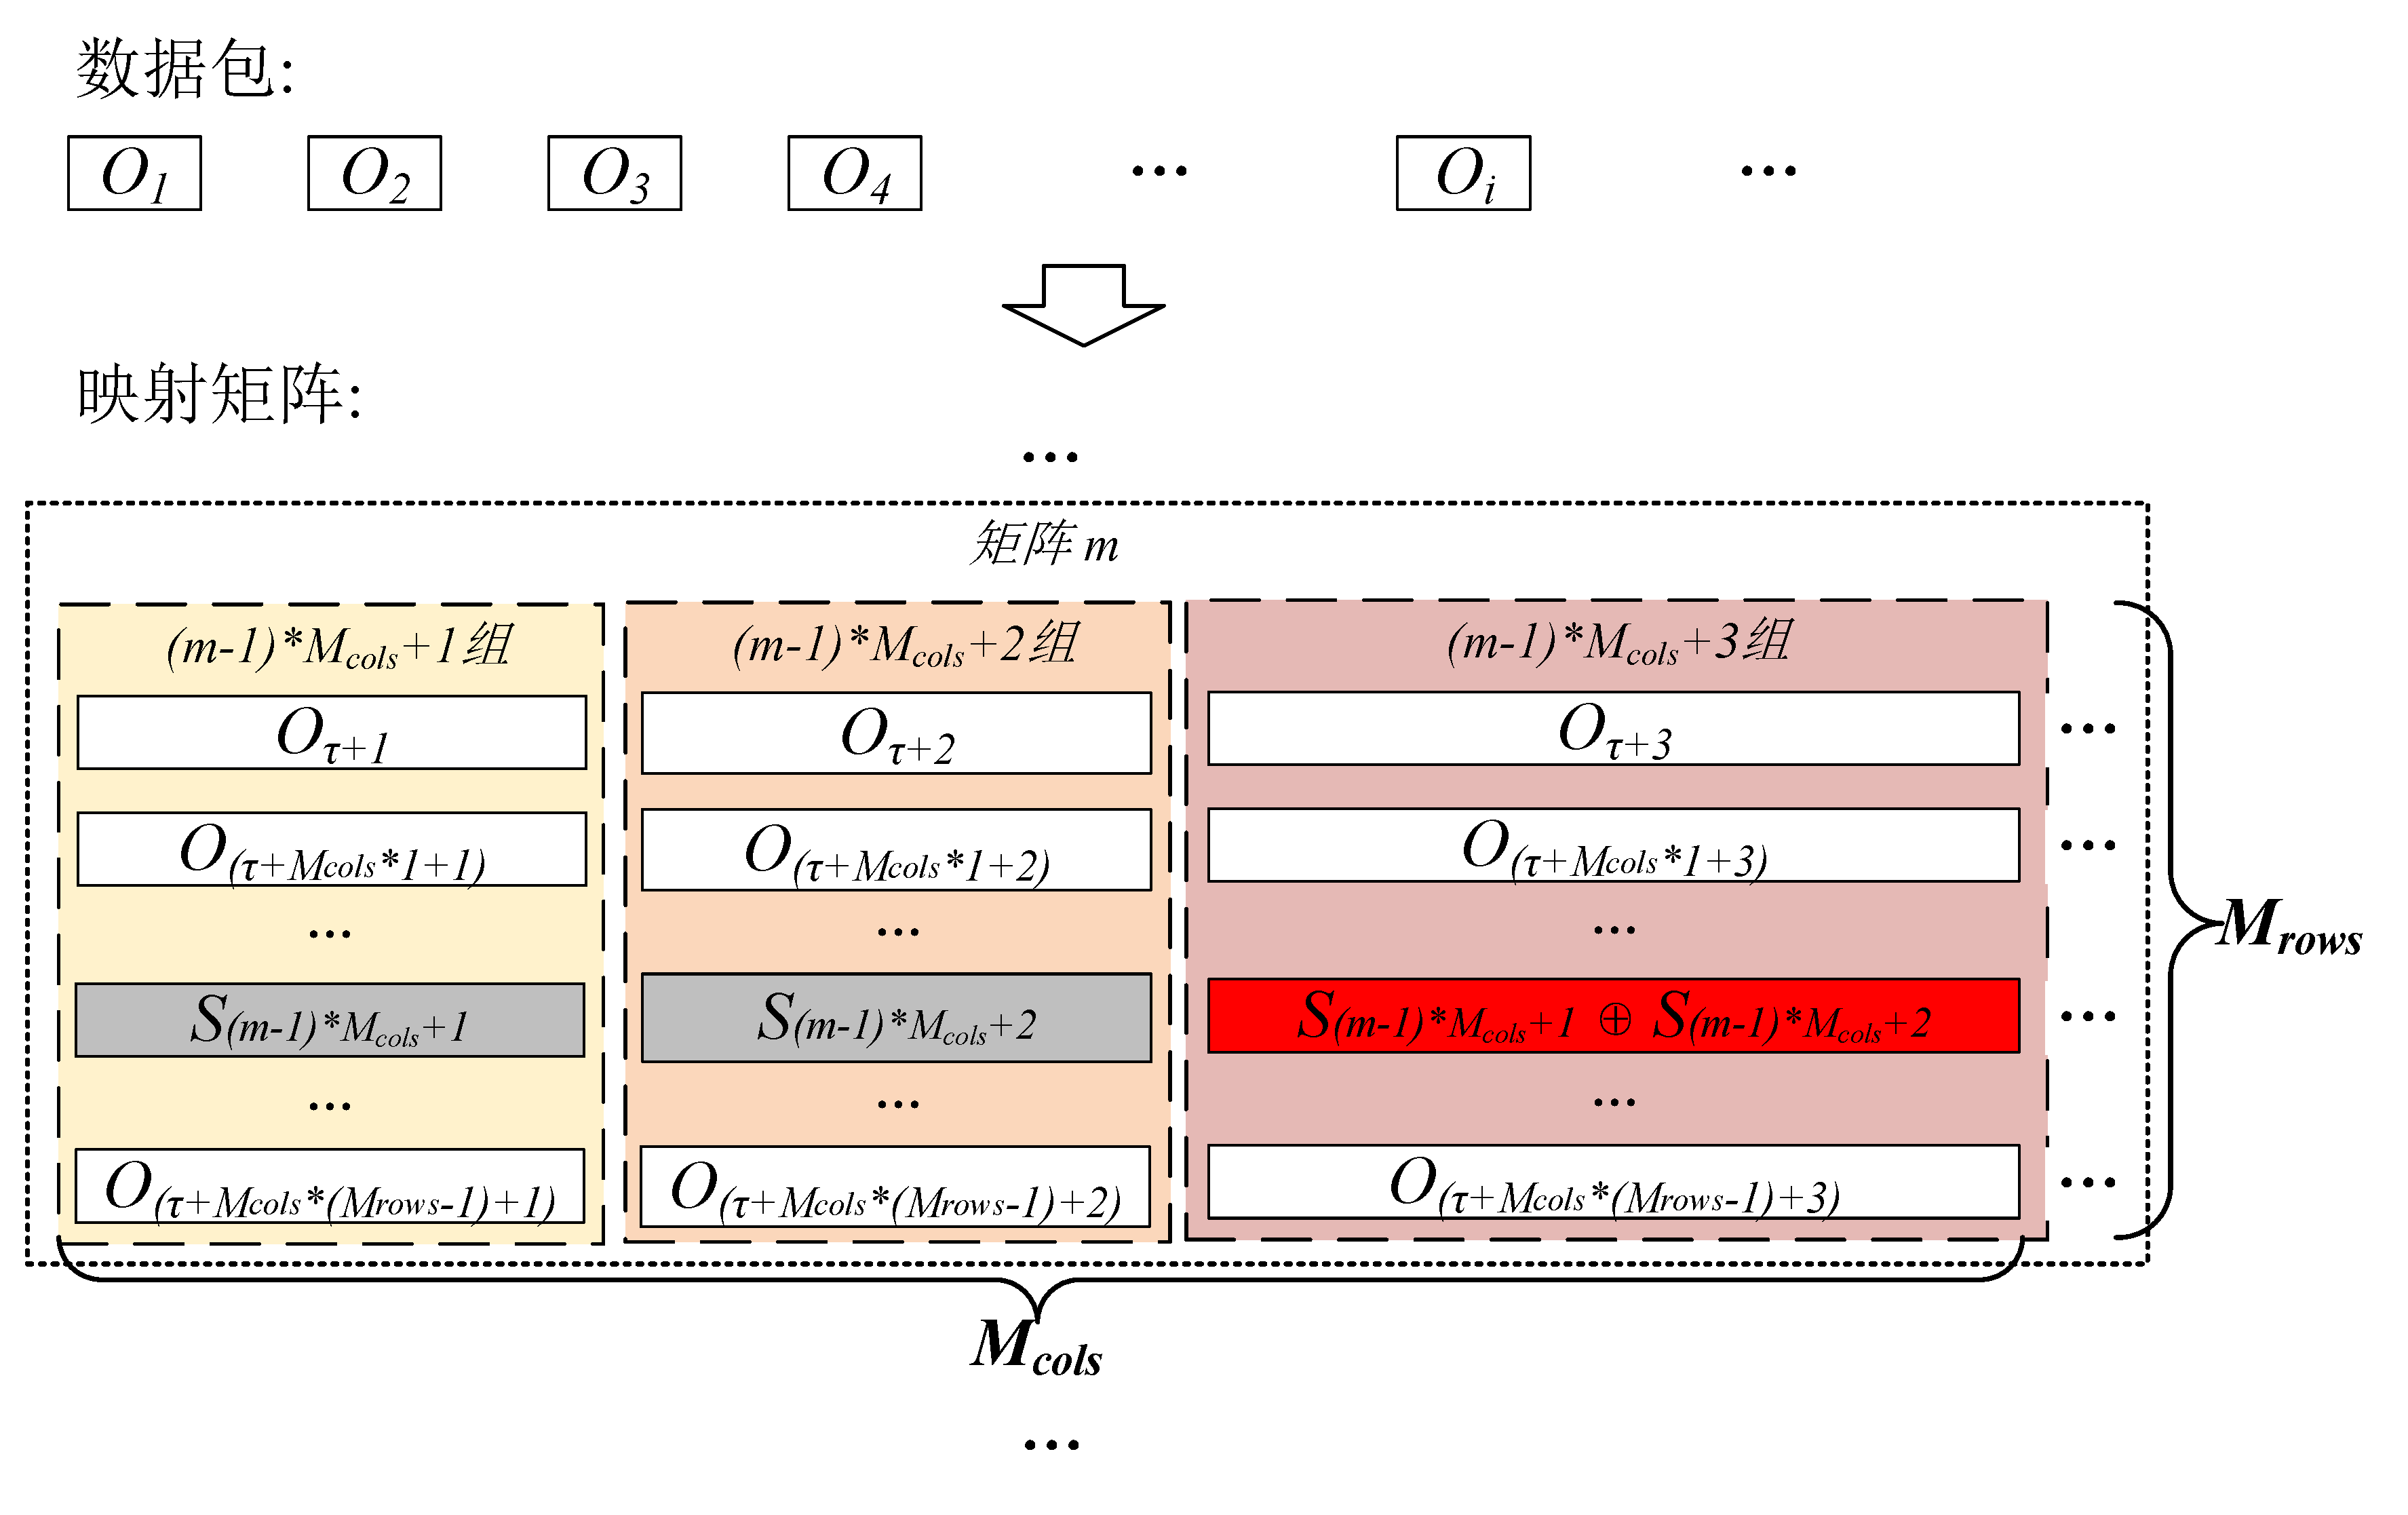
\includegraphics[width=0.95\textwidth]{chapters/chapter5/figures/mapping-matrix.pdf}
        \caption{映射矩阵及异或校验示意图}
        \label{fig:5:mapping-matrix}
    \end{figure}
}

映射矩阵及矩阵中的异或校验如图\ \nref{fig:5:mapping-matrix}所示,数据包序号按照行序填充矩阵。对于第$m$个映射矩阵,矩阵由$O_{\tau\ +\ 1}$开始,其中$\tau$由公式(\nref{equ:5:tau})定义。矩阵的行数$M_{rows}$与符号的表示范围有关,$M_{rows}$由公式(\nref{equ:5:m-rows})根据$L_{Codeword}$计算得出。
\insertEquation{
    \begin{equation}
        \label{equ:5:m-rows}
        M_{rows}\ =\ 2^{L_{Codeword}}
    \end{equation}
    \begin{equation}
        \label{equ:5:tau}
        \tau\ =\ M_{cols}\ \times\ (m\ -\ 1)\ \times\ M_{rows}
    \end{equation}
    \begin{equation}
        \label{equ:5:p_k}
        P_k\ (k,\ S_k)\ =\ \left \lfloor{\frac{k\ -\ 1}{M_{cols}}}\right \rfloor \times (M_{rows} \times M_{cols})\ +\ M_{cols} \times (S_k\ -\ 1)\ +\ (k\ -\ 1)\ \%\ M_{cols}\ +\ 1
    \end{equation}
}
\insertContents{
    \begin{algorithm}[htbp]
        \renewcommand{\algorithmcfname}{算法}
        \caption{码字转换为序号}
        \label{alg:5:codeword-to-sequence}
        \LinesNumbered
        \KwIn{$C$,\ $L_{Codeword}$,\ $M_{cols}$,\ $Salt$,\ $Seed$}
        \KwOut{$P\ \leftarrow\ \{\}$}
        $S\ \leftarrow\ \{\}$ \\
        $offset\ \leftarrow$\ Random\ ($Salt\ \oplus\ Seed$) \\
        \For {$C_j$ in $C$} {
            $S_k\ \leftarrow$\ Integer\ ($C_j$)\ +\ 1 \\
            append\ $S_k$\ to\ $S$ \\
            \If {$j$\ mod\ 2\ ==\ 0} {
                append\ ($S_k\ \oplus\ S_{k-1}$)\ to $S$
            }
        }
        \For {$S_k$\ in\ $S$} {
            $offset\ \leftarrow$\ Random\ ($offset$) \\
            $S_k\ \leftarrow\ (S_k\ +\ offset)\ mod\ (2^{L_{Codeword}})\ +\ 1$
        }
        \For {$S_k$\ in\ $S$} {
            $P_k\ \leftarrow\ P_k\ (k,\ S_k)$ \\
            append\ $P_k$\ to\ $P$
        }
        \Return $P$
    \end{algorithm}
}

映射矩阵中,每一个数据包序号均有其坐标值,纵坐标代表符号,横坐标为分组序号。映射矩阵中,基于异或校验的校验符号,每两个数据符号则插入一个。如图\ \nref{fig:5:mapping-matrix},第$(m-1)\ \times\ M_{cols}\ +\ 3$组需要添加异或校验符号,则插入前两组符号的异或值$S_{(m\ -\ 1)\ \times\ M_{cols}\ +\ 1}\ \oplus\ S_{(m\ -\ 1)\ \times\ M_{cols}\ +\ 2}$。异或校验关系每3个符号一组,要求$M_{cols}\ \%3\ =\ 0$,从而映射矩阵与异或校验周期同步。

码字到数据包序号的转换过程,如算法\ \nref{alg:5:codeword-to-sequence},输入参数包括码字集合、传输参数及随机数种子。首先根据$Salt$及$Seed$生成随机数种子,第一步添加异或校验,第二步添加随机偏移量,第三步将符号转换为序号,三步各对应一轮循环。

第一步添加异或校验,判断进行到偶数组时,将前两组符号异或,然后加入到符号集合$S$。第二步添加随机偏移量,每次迭代伪随机数发生器,从而即使是相同的符号,对应的处理结果也不完全相同。第三步将符号映射到序号,符号及组号构成$[k,\ S_{k}]$二元组,按照公式(\nref{equ:5:p_k}),转换为数据包序号。

\subsubsection{解调阶段}
\label{chap:hash:robustness:xor:demodulation}
\insertEquation{
    \begin{equation}
    \label{equ:5:get-k}
        k\ =\ \left \lfloor{\frac{P'}{M_{rows}\ \times\ M_{cols}}}\right \rfloor\ \times\ M_{cols}\ +\ (P'\ -\ 1)\ \%\ M_{cols}\ +\ 1
    \end{equation}
    \begin{equation}
    \label{equ:5:get-s}
        S_j'\ =\ \left \lfloor{\frac{P_j'\ -\ M_{rows}\ \times\ M_{cols}\ \times\ \left \lfloor{\frac{P_j'}{M_{rows}\ \times\ M_{cols}}}\right \rfloor\ -\ 1}{M_{cols}}}\right \rfloor
    \end{equation}
    \begin{equation}
    \label{equ:5:remove-offset}
        S_j'\ =\ ({S_j'\ -\ offset\ \%\ ({2^{L_{Codeword}}})\ +\ 2^{L_{Codeword}}})\ \%\ (2^{L_{Codeword}})\ +\ 1
    \end{equation}
}

解调过程中,参照映射矩阵提取符号信息,同时对异或校验符号进行验证。接收方获取丢包序号$P'$,根据公式(\nref{equ:5:get-k})计算组号,通过公式(\nref{equ:5:get-s})提取出候选符号。受噪声影响,每一组的候选符号不唯一,因此得到的结果为$\{\{S_1',\ \cdots\}$, $\{S_2',\ \cdots\}$, $\cdots$, $\{S_k',\ \cdots\}$, $\cdots\}$。

对于候选符号,首先消除随机偏移量,该过程如公式(\nref{equ:5:remove-offset})。其中,每一组的$offset$通过迭代伪随机数发生器获取,与调制阶段相同。通过验证符号间的异或校验关系,即可完成多层校验的第一层校验。校验过程中利用异或关系的特征,当符号$S_1',\ S_2',\ S_3'$满足$S_1'\ \oplus\ S_2'\ \oplus\ S_3'\ =\ 0$时,判断符合校验规则。